\documentclass{article}
\setlength{\textwidth}{6.2in}
\setlength{\oddsidemargin}{0in}
\setlength{\evensidemargin}{0in}
\setlength{\textheight}{8.7in}
\setlength{\topmargin}{0in}

\usepackage{graphicx}
\usepackage{mathtools}
\usepackage{cite}

\begin{document}

\begin{center}
\huge{Uncertainty Quantification Plan}
\end{center}

\vspace{0.2in}

\section{Introduction}

The Plasma-Surface-Interactions (PSI) SciDAC project is focused on predictive
modeling of material damage in the tungsten wall material of the plasma divertor
in a Tokamak fusion reactor system. The effort includes multiscale modeling
methodologies involving particle in cell (PIC) methods, molecular dynamics (MD),
and continuum modeling. For the latter, a high performance simulator named
Xolotl is being developed.

Xolotl is able to reproduce the evolution of the surface of the material by
solving the cluster dynamics formulated Advection-Diffusion-Reaction (ADR)
equations with an incident flux
\begin{equation}
	\delta_t \bar{C} = \phi \cdot \rho + D \nabla^2 \bar{C} - \nabla \bar{\nu}C -
	\bar{Q}(\bar{C})
\end{equation}

The time evolution of the concentration of each cluster in the network
($\delta_t \bar{C}$ where $\bar{C}$ is the vector of concentrations) is thus
related to the external flux ($\phi \cdot \rho$), the isotropic diffusion ($D
\nabla^2 \bar{C}$), the advection ($\nabla \bar{\nu}C$), and the reactions
between the clusters ($\bar{Q}(\bar{C})$). In order to compute these different
quantities, one needs different input information.

The diffusion coefficient is a function of the diffusion factor
$D_0$ and the migration energy $E_m$
\begin{equation}
	D_i = D_{0,i} \cdot e^{-E_m/(k_B T)}
\end{equation}
with $k_B$ the Boltzmann constant and $T$ the temperature.

The reactions between clusters can be separated into two categories: actual
reaction $r_i$ (where the cluster $i$ is produced or is used to produce another
cluster) and dissociation $d_i$ (where the cluster $i$ is dissociated in two
other clusters). The former quantity is a function of all the concentrations,
$\bar{C}$, and of the diffusion coefficient $D_0$, while the latter is a
function of the binding energies $E_b$ in addition to the previous quantities. The
details of the aforementioned functions will not be explained here, but the
curious reader can have a look at this
document \cite{math} for more information.

The advection part is not yet taken into account here and the external flux is
a constant. \newline

Most of the quantities that are needed ($E_b$, $E_m$, $D_0$) are results of
simulations combined with experimental observations and, as a consequence, are
not perfectly determined. In order for Xolotl to give more relevant results, one
has to explore the influence of these uncertainties on the final result. This
will be done with the help of Uncertainty Quantification (UQ) techniques.

\section{Uncertainty Quantification Techniques}

Before being able to perform any uncertainty quantification, one needs to have
some knowledge about the underlying concepts. This section is devoted to the
description of the main concepts that will be used to quantify the
uncertainties occurring in Xolotl.

\subsection{Bayesian Inference}

Inference refers to the process of deriving logical conclusions from premises
assumed to be true. Bayesian inference is thus the same idea which uses Bayes'
rule for the process. Three important quantities take part in that rule:
\begin{equation}
	P(H|E) \propto P(E|H) \cdot P(H)
\end{equation}

\begin{itemize}
  	\itemsep0em
  	\item[-] the posterior $P(H|E)$ (probability of the hypothesis $H$ given the
  	evidence $E$) that is infered;
  	\item[-] the likelihood $P(E|H)$ (probability of the evidence $E$ given the
  	hypothesis $H$);
  	\item[-] and the prior $P(H)$ that gathers all the information one had before
  	the evidence $E$ was observed.
\end{itemize}

This simply means that the posterior is updated from the prior for each
occurence of new evidence observed, knowing the likelihood of observing
these evidences given the hypothesis. \newline

The important feature of Bayesian inference is that everything is considered as
a random variable. For instance, if one is given a number of data points and
wants to model them with a line, the probability density functions (PDF) for
each coefficient of the polynomial would need to be initially specified.
These PDFs are the priors and do not need to be well defined. Furthermore,
this lack of knowledge can be shown by simply using a flat PDF (e.g. a
uniform distribution along the interval $[-1000,1000]$ for each
coefficient).
The likelihood function is a direct derivative of the model that is used for the inference. \newline

Most of the time, the posterior cannot be calculated analytically because of its
integral form. Markov Chain Monte-Carlo (MCMC) is a method used to tackle this
problem, where a Markov chain randomly wanders in the parameter space.
The PDF of the posterior is then obtained gathering the steps taken by the
Markov chain.

\subsection{Global Sensitivity Analysis}

Global sensitivity analysis is a technique that is commonly used with the
intentions of reducing model dimensionality.  Performing a global sensitivity
analysis determines an influential hierarchy of uncertain input parameters in
relation to the variation of the output.  The aforementioned hierarchy, thus,
enables the identification of the input parameters whose uncertainty has a
negligible contribution to uncertainties in the quantities of interest. \newline

Let $i \subseteq \mathcal{I} = \{ 1,\ldots,n\}$.  Assume $\boldsymbol{\xi}$ to
be the set of uncertain model input parameters such that $\boldsymbol{\xi} \in
\mathcal{U}^n$  where $\mathcal{U}^n = \{\boldsymbol{\xi} :
0 \leq \xi_i \leq 1, i \in \mathcal{I}\}$ is the $n$-dimensional hypercube.
Suppose $f$ represents the model output which can be denoted by \ref{eq:pce}.

The mean value, or expectation of $f$, is defined by
\[
f_0 = E(f) =
\int_{\mathcal{U}^d} f(\boldsymbol{\xi})d\boldsymbol{\xi}
\]
Additionaly,
\[
 f_i(\xi_i) = E(f|\xi_i)- f_0
= \int_{\mathcal{U}^{d-1}} f(\boldsymbol{\xi})d\boldsymbol{\xi}_{\sim i} - f_0
\]
defines the conditional expectation, or first order effect, where $\xi_{\sim i}$
denotes the set of all input parameters except $\xi_i$.  This describes the
effect on the model output that results from varying $\xi_i$.
\newline

Analogous to the first order definition, the second order effect,
$$ f_{ij}(\xi_i,\xi_j) = E(f|\xi_i,\xi_j) - f_0 - f_i - f_j $$
defines the effect on the model output that results from simultaneously varying
$\xi_i$ and $\xi_j$ along with their corresponding individual effects. \newline

There are two quantities that are of particular importance when performing
a global sensitivity analysis: first order sensitivity indices and total
sensitivity indices.  First order sensitivity indices (sometimes referred to as
main effect sensitivity indices), $S_{i}$, describe the fraction of the
uncertainty in the output, $f$, that can be attributed to the input parameter
$\xi_i$ alone. This quantity compares the variance \cite{spectral} of
the conditional expectation, $Var[E(f|\xi_i)]$, against the total variance,
$Var(f)$, i.e.
\begin{equation}
      S_i = \frac{Var[E(f|\xi_i)]}{Var(f)}
      \label{eq:si}
\end{equation}
%   \begin{equation}
%    S_i =
%    \frac{\sum_{k \in \mathbb{I}_i} f_k^2 \| \varphi_k \|^2}{\sum_{k=1}^P f_k^2 \| \varphi_k \|^2} = \frac{\sum_{k \in \mathbb{I}_i}
%   f_k^2 \| \varphi_k \|^2}{Var[f({\boldsymbol \xi})]}
%   \end{equation}
%   where $\mathbb{I}_i$ are the terms involving $\xi_i$ only. \newline
%   AKA 1st order main effects
%   \item {\bf Joint sensitivity indices} (uncertainty contribution due
%   to terms with only $\xi_i\xi_j$)
%   \begin{equation}
%   S_{ij} = \frac{ \sum_{k \in \mathbb{I}_{ij} } f_k^2 \|
%   \varphi_k \|^2 }{ \sum_{k=1}^P f_k^2 \| \varphi_k \|^2 }
%   \end{equation}
%   where $\mathbb{I}_{ij}$ are the terms involving $\xi_i\xi_j$ only

Total sensitivity indices, $T_i$, describe the contribution to the uncertainty
in the model output resulting from the uncertain input $\xi_i$ including all
corresponding interactions with other input variables, 
\begin{equation}
      T_i = \frac{E[Var(f|\boldsymbol{\xi}_{\sim i})]}{Var(f)} =
      \frac{Var(f) - Var[E(f|\boldsymbol{\xi}_{\sim i})]}{Var(f)}
\end{equation}

\subsection{Polynomial Chaos Expansion}

Polynomial chaos expansion (PCE) is a method used to represent uncertain
quantities of interest (QoIs) in terms of orthogonal polynomials with
independent random variables (RVs) with known densities. \newline

% Let $\boldsymbol \xi$ be a set of $n$ independent random variables, with known
% densities, which parameterize the uncertain input quantities.  Clearly, the
% output $f$ is dependent upon the random inputs which, in turn, results in the
% output being random. 

Let $\boldsymbol \xi$ be a set of $n$ independent random variables, with known
densities, for which the QoI $f$ is dependent upon.  Assuming $f$ is
square-integrable, it can be represented by the polynomial chaos expansion
\begin{equation}
    f(\boldsymbol{\xi}) = \sum_{k=0}^P f_k\varphi_k(\boldsymbol \xi)
    \label{eq:pce}
\end{equation}
where $\varphi_k$ are the $n$-dimensional basis functions up to order P with
coefficients $f_k$.

Utilizing the orthogonality of the basis functions, the deterministic
coefficients $f_k$ are simply given by

\begin{equation}
    f_k = \frac{\langle
    f,\varphi_k \rangle}{\| \varphi_k \|^2} \text{,  } \; k=0,\ldots,P
\end{equation}

The choice of the polynomial chaos (PC) type to be used often depends
principally on the domain of input parameters, even if the PDF of these
parameters can also be mapped to any given known density (gaussian, uniform,
gamma, beta, \dots).

\section{Initial Investigation of Input Parameters}
\subsection{Parameters Under Consideration}

In the first phase of Xolotl, only the one-dimensional case of the ADR equations
for tungsten is considered. For this problem, the clusters are composed of
three different elementary clusters: helium (He), vacancy (V), and interstitial
(I). Each cluster is defined by its composition ($n_{He}$, $n_V$, $n_I$),
binding energies ($E_{b, He}$, $E_{b, V}$, $E_{b, I}$), migration energy
($E_m$), and diffusion coefficient ($D_0$). \newline

A text file containing the information for each cluster in the network is
currently being used as an input for Xolotl. This means that when looking at
small networks considering only ten clusters, the number of input parameters
is fifty.

Luckily, binding energies can actually be computed from formation energies
through the formula
\begin{eqnarray}
    E_{b, He}(He_X, V_Y, I_Z) & = & E_f(He_{X-1}, V_Y, I_Z) + E_f(He_1, 0, 0) -
    E_f(He_X, V_Y, I_Z) \nonumber \\
    E_{b, V}(He_X, V_Y, I_Z) & = & E_f(He_X, V_{Y-1}, I_Z) + E_f(0, V_1, 0) -
    E_f(He_X, V_Y, I_Z) \\
    E_{b, I}(He_X, V_Y, I_Z) & = & E_f(He_X, V_Y, I_{Z-1}) + E_f(0, 0, I_1) -
    E_f(He_X, V_Y, I_Z) \nonumber
\end{eqnarray}

Using the formation energies as an input would then reduce the number
of parameters from five to three for each cluster. \newline

At the moment, formation energy data is only available for $HeV$ clusters with
$V = 1, 2, 6, 14, 18, 19,$ $27, 32, 44$ (for tungsten problems, one is mainly
interested in $HeV$ clusters with $V$ up to $50$). Figure \ref{fig:Ef} shows
the formation energy data as a function of the helium and vacancy cluster sizes.
By representing this as a function of the helium/vacancy ratio, one can see
common features appearing.

\begin{figure}[!htbp]
      \begin{center}
        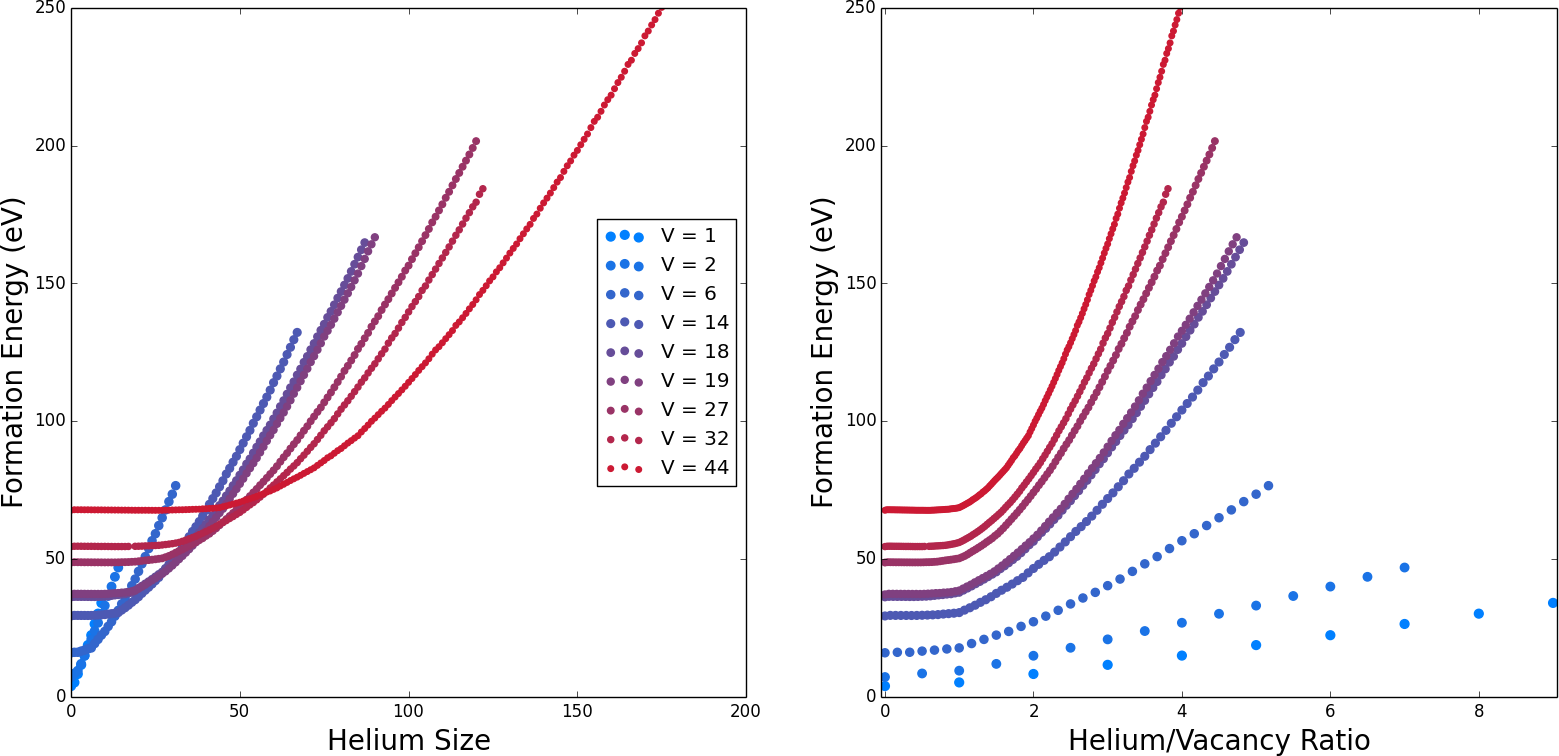
\includegraphics[width=0.95\textwidth]{formationEnergiesUQ}
        \caption{Formation energies (in eV) for $V = 1, 2, 6, 14, 18, 19, 27, 32,
        44$ as a function of the number of helium in the cluster (left) of the
        helium/vacancy ratio (right). \label{fig:Ef}}
      \end{center}
\end{figure}

Modeling the formation energies would permit extrapolation of the missing data
and, additionally, would result in a drastic reduction of the number of input
parameters.

\subsection{Modeling the Formation Energies}

The first step in the modeling of the formation energies is to find a good fit.
This fit function will depend on both helium and vacancy sizes (even
though the representation in figure \ref{fig:Ef} can be misleading). Also, a
change of variable from the helium size to the helium/vacancy ratio seems
to be more suitable in order to capture the formation energy features.  This
data clearly captures the existence of two different behaviours separated at
helium/vacancy ratio around one. The use of a piecewise function for the fit is
thus indicated. \newline

Once this fit is obtained, a thorough investigation of the difference between
the data and the fit will be necessary. In turn, this will help shape the
existing uncertainties of the model (standard deviation and/or bias). \newline

Then, the Bayesian Inference method can be used to infer the final model of the
formation energies and the joint posteriors (giving information about the
correlation between parameters). The coefficients of the fit function will be
used as the parameters (priors), and the uncertainties of the model will be
considered as hyperparameters (hyperparameter meaning parameter of the prior). 

This will be done with the help of the UQ Toolkit \cite{uqtk} libraries
providing (among others) a Bayesian Inference method using a Metropolis-Hastings
MCMC algorithm. After which, the obtained joint posterior would, nearly, be
ready for use in other UQ methods.

\section{Proposed Strategy}

This section starts with the description of the quantities of interest under
consideration, and then exhibits the different methods that are planned to be
used to perform uncertainty quantification on the Xolotl software. The
DAKOTA \cite{dakota} software was chosen as the provider of these algorithms.

\subsection{Quantities of Interest}

To be determined\dots

\subsection{Global Sensitivity Analysis}

A global sensitivity analysis will be done on Xolotl in order to determine
the influential hierarchy of the uncertain input parameters and to reduce
the overall model dimensionality. 

Two independent ways to do so are considered in the following sections.

\subsubsection{Obtaining Sensitivity Indices via Monte-Carlo Sampling}

This method is a computationally expensive one. Random variations of the input
parameters will be generated and the Xolotl software will be run for each of variations.

Monte-Carlo sampling will be used first for global sensitivity analysis in order
to have a rough estimate of the important input parameters. A more refined
analysis will be then performed with the use of a PC surrogate (see next
section). \newline

Let $X = \{\boldsymbol{\xi}^{(1)}, \ldots, \boldsymbol{\xi}^{(M)}\}$ and
$\tilde{X} = \{\boldsymbol{\xi}^{(1)}, \ldots, \boldsymbol{\xi}^{(M)}\}$ be
independent sample sets drawn uniformly in $\mathcal{U}^d$.

It follows that one can estimate the mean, $E(f)$, and
variance, $Var(f)$, respectively as follows (where the hat denotes the
estimator)
\begin{equation}
	\widehat{E(f)} = \frac{1}{M} \sum_{s=1}^M f(\boldsymbol{\xi}^{(s)})
\end{equation}
\begin{equation}
	\widehat{Var(f)} = \frac{1}{M-1} \sum_{s=1}^M [f(\boldsymbol{\xi}^{(s)})]^2 -
	\widehat{E(f)}^2
\end{equation}

Utilizing the previous results and equation (\ref{eq:si}), it can be shown that
the first order sensitivity indices are estimated \cite{sobol} by
\begin{equation}
	\widehat{S_i} =
	\frac{Var[\widehat{E(f|\xi_i)}]}{\widehat{Var(f)}}
\end{equation}
where 
\[
	Var[\widehat{E(f|\boldsymbol{\xi}_i)}] = \frac{1}{M}
	\sum_{s=1}^M f(\boldsymbol{\xi}^{(s)}_{\sim i},\boldsymbol{\xi}^{(s)}_i)
	f(\boldsymbol{\tilde{\xi}}^{(s)}_{\sim i},\boldsymbol{\xi}^{(s)}_i) -
	\widehat{E(f)}^2 .
\]

Analogously,
\begin{equation}
	\widehat{T_i} = 1 - \frac{Var[\widehat{E(f|\boldsymbol{\xi}_{\sim
	i})}]}{\widehat{Var(f)}}
\end{equation}
estimates the total sensitivity indices with
\[
	Var[\widehat{E(f|\boldsymbol{\xi}_{\sim i})}] = \frac{1}{M}
	\sum_{s=1}^M f(\boldsymbol{\xi}^{(s)}_{\sim i},\boldsymbol{\xi}^{(s)}_i)
	f(\boldsymbol{\xi}^{(s)}_{\sim i},\boldsymbol{\tilde{\xi}}^{(s)}_i) -
	\widehat{E(f)}^2  .
\]

\subsubsection{Obtaining Sensitivity Indices via PCE}

The perks of using PCE to represent quantities of interest is that parametric
sensitivity information comes as a direct result. It is simply a matter
of taking the PCE and decomposing it termwise.  

To illustrate this, $f \in \mathcal{L}_2(\mathcal{U}^n)$ will be represented by
(\ref{eq:pce}) as follows
\[
	f({\boldsymbol \xi}) = \sum_{k=0}^P f_k\varphi({\boldsymbol \xi}) .
\]

The mean, or expectation, of $f$ is defined to be 
\[
	E(f)=f_0 ,
\]
and the variance
\[
   \sigma^2 =
    Var[f({\boldsymbol \xi})] = \sum_{k=1}^P f_k^2 \| \varphi_k \|^2
\]
From the previous definition, and recalling (\ref{eq:si}), it follows that the
first order sensitivity indices are determined by
\begin{equation}
  	S_i = \frac{\sum_{k \in \mathcal{I}_i}f_k^2 \| \varphi_k
  \|^2}{Var[f({\boldsymbol \xi})]}
\end{equation}
where $\mathcal{I}_i$ are the terms involving $\xi_i$ only.
The joint sensitivity indices, uncertainty contribution due to terms
with only $\xi_i\xi_j$, are similarly obtained.  Hence,
\[
	S_{ij} = \frac{\sum_{k \in \mathcal{I}_{ij}} f_k^2 \| \varphi_k
	\|^2}{Var[f({\boldsymbol \xi})]}
\]
where $\mathcal{I}_{ij}$ are the terms involving $\xi_i\xi_j$ only.
Recall that the total sensitivity indices describe the uncertainty contribution
due to all terms containing $\xi_i$; thus $T_i$ can be obtained by simply
summing all sensitivity indices involving $\xi_i$.

\subsection{Constructing Xolotl Surrogate}

A surrogate model is an inexpensive approximate model intended to capture the
salient features of an expensive high-fidelity model. It can be built
directly from data (QoIs) generated by Xolotl here. \newline

Given the supposed strong nonlinear dependence of the system on uncertain
parameters, and because the solution typically exhibits the formation of sharp fronts, it is
advisable to consider non-intrusive PC methods, focusing on smooth observables,
and relying on sparse quadrature sampling. \newline

Xolotl's output quantities of interest will be approximated using the theory of
polynomial chaos expansions previously defined.  Representing these quantities
as such enables the construction of PC surrogates for the QoIs. Employing a
Non-Intrustive Spectral Projection (NISP) method, a projection is applied
exclusively to the QoIs and thereby only computing PCEs for these quantities.
Using the NISP method allows Xolotl to be used as a black box in order to obtain
function evaluations from which the PC coefficients are determined. \newline

To illustrate this idea, let $y = f(\boldsymbol{\xi})$ be an output QoI in
Xolotl and $\boldsymbol{\xi}$ be the set of uncertain parameterized inputs.
The output will be represented with a PCE as shown in (\ref{eq:pce}). Recall
that the deterministic coefficients are found by
\[
f_k=\frac{\langle f,\varphi_k \rangle}{\| \varphi_k \|^2}
= \frac{\int f\varphi_k(\xi)w(\xi)d\xi}{\int \varphi_k^2(\xi)w(\xi)d\xi} \text{,
} \; k=0,\ldots,P
\]

These integrals will be evaluated using numerical quadrature,
\[
 \int f\varphi_k(\xi)w(\xi)d\xi=\sum_{q=1}^Q w_q f(\xi_q)\varphi_k(\xi_q)
\]
where $\xi_q$ and $w_q$ are the multidimensional quadrature points and
weights, respectively, and $Q$ is the number of 1D quadrature points. Such
standard quadrature methods use tensor products of the 1D quadrature rules which
require, approximately, $Q^n$ computations in order to evaluate the integrals. 
\newline

The high dimensionality of Xolotl suggests an optimal alternative to standard
numerical quadrature would be to use adaptive sparse quadrature methods, the
details of which can be found in \cite{spectral}.
      
\section{In a Nut Shell\dots}

The Xolotl uncertainty quantification plan is as follows: the first step would
be a Monte-Carlo sampling based global sensitivity analysis to establish which
uncertain inputs matter; then, a PC surrogate for the quantities of interest
would be constructed using adaptive sparse quadrature; finally, the
input paramaters uncertainties (previously determined with the help of
Bayesien inference) can be propagated through Xolotl with using the
PC surrogate via Monte-Carlo.

\bibliographystyle{plain}
\bibliography{biblio}

\end{document}